\section{Computational Assistance Across Analytic Workflows}
\label{sec:assistance}

Computational assistance changes both the objects available for analysis and the actions through which scientists investigate them. A computed layout makes relationships inspectable; a classifier propagates labels beyond the examples an expert has examined; a language interface translates a question into operations. The four assistance modes introduced in Section~\ref{sec:foundations} distinguish these contributions without assigning each system to a single category. We compare mechanisms by their inputs, computational behavior, outputs, and opportunities for human intervention. Tasks provide the purpose of that intervention, while the locus of analytic agency explains which decisions the scientist retains, supplies indirectly, or delegates.

Figure~\ref{fig:assistance-modality-map} maps representative systems across assistance modes and visualization environments. A system may occupy several cells when it combines multiple forms of assistance or supports multiple environments.

\subsection{Algorithmic Assistance: Transforming the Analytic Substrate}
\label{sec:assistance-algorithmic}

Algorithmic assistance establishes structures on which subsequent interpretation is based. Clustering and dimensionality reduction organize similarities; layout and aggregation make relationships tractable; annotation and ranking connect observations to candidate explanations. These transformations make selected properties easier to inspect while placing others outside the immediate view. Their analytical consequences therefore depend on how scientists choose inputs, inspect results, and relate computed structure to the underlying evidence. Dimensionality reduction illustrates this distinction. Espadoto et al. survey projection techniques using criteria including preservation of data structure, scalability, and robustness.~\cite{espadoto2021quantitative} These criteria help compare the computational transformation; evidence that a projection supports a particular biological interpretation must be assessed separately.

RNA-SeqEZPZ integrates quality control, alignment, counting, differential-expression analysis, and pathway analysis behind a Shiny interface. Scientists supply files and parameters, initiate the pipeline, and explore outputs through interactive views. The mechanism delegates execution of a configured sequence while leaving its purpose and interpretation with the scientist.~\cite{AnchorRNASeqEZPZ} PeCaX connects somatic-variant annotation and pathway-network construction to filtering, inspection, and annotation for molecular-tumor-board work.~\cite{AnchorPeCaX} Here, assistance makes relationships among variants, pathways, and treatment evidence available for consideration; it does not itself establish which interpretation should guide a clinical decision.

\begin{figure*}[t]
\centering
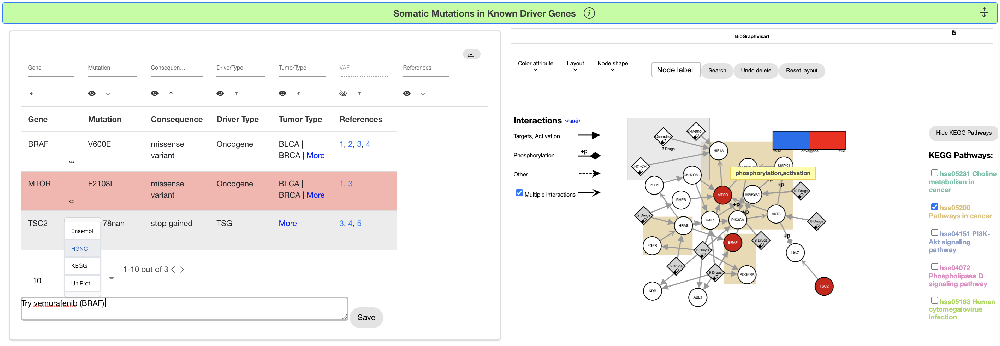
\includegraphics[width=\textwidth]{figures/system-examples/pecax_variant_network.pdf}
\caption{PeCaX connects annotated patient variants with gene--drug network context. The table summarizes somatic mutations in known driver genes, including predicted consequences, driver types, and reference sources; the associated network places affected genes alongside interacting genes and drugs, with controls for inspecting pathway context. Algorithmic annotation and network construction provide evidence that scientists can inspect when interpreting molecular findings. Cropped from Fig.~2 (upper table--network pair) in Additional file~1 of Figaschewski et al.~\cite{AnchorPeCaX}. \copyright{} The Author(s) 2023, licensed under CC BY 4.0 (\protect\url{https://creativecommons.org/licenses/by/4.0/}); cropping only.}
\label{fig:pecax-variant-network}
\end{figure*}


Representation-oriented systems expose a different point of intervention. Compressed Adjacency Matrices combine computational organization of gene regulatory networks with analyst-controlled rearrangement, highlighting, and filtering.~\cite{AnchorCompressedMatrices} Flud combines crowd-worker node placement with computational scores, clues, and simulated annealing.~\cite{bharadwaj2022flud} The comparison concerns how representational changes are distributed among analyst interaction, crowd work, and automated search. Flud’s layout and task results support its optimization strategy; an effect on biological discovery remains to be evaluated. Across these systems, the relevant question is what the transformation enables scientists to examine and how its assumptions remain available for scrutiny.

The same execution pattern appears in iGEAK, BioNetApp, OncoProExp, and SeqPlots: normalization, statistical comparison, clustering, aggregation, or pathway analysis remains connected to interactive inspection.~\cite{ExpandedE38,ExpandedE39,ExpandedE47,ExpandedE44} VIADS adds hierarchical aggregation and threshold-revisable summaries, while LIM Tracker couples automated tracking to manual correction and rerunning.~\cite{ExpandedE40,ExpandedE32} Virtual embolization instead lets analysts compare simulated occlusion alternatives on desktop and in VR.~\cite{ExpandedE30} These are distinct analytical substrates, not interchangeable demonstrations of autonomy.


\subsection{Adaptive Assistance: Responding to Analysis State}
\label{sec:assistance-adaptive}

Adaptive assistance depends on a relationship between an observed signal and a subsequent computational intervention. The signal may concern user feedback, developing task context, or data characteristics; the intervention may revise a model, prioritize candidates, or change guidance. Adaptation need not involve learned personalization, but it must be distinguished from simply exposing adjustable parameters. The useful comparison identifies what changes, why it changes, and how the scientist can influence that change.

Four questions make an adaptive mechanism explicit: what signal is observed, how it is used directly or interpreted as analytic context, what computational intervention changes in response, and what controls are available to the scientist. Signals may include explicit feedback, interaction history, task context, or data uncertainty; inferred goals and persistent user models are not required. Inspection, rejection, and reversal should be described as implemented capabilities where documented, and otherwise as design requirements. This account distinguishes what the system observes from what it assumes. Dwell time, for example, could indicate interest, confusion, or interruption; recording it does not establish that any one interpretation is correct.

Algorithmic processing and adaptation can consequently be coupled: a transformation produces candidate structures, while feedback or contextual information influences subsequent computation or presentation. The distinction does not depend on who initiates execution. Scientists may request adaptive guidance, and a fixed algorithmic pipeline may execute automatically. Nor is adaptation necessarily persistent learning: a context-dependent intervention and a model updated from feedback require different descriptions.

Facetto provides a concrete feedback loop. Experts inspect multiplex images and coordinated feature views, select regions and features, examine clusters, and revise phenotype labels. Those labels feed a classifier whose subsequent assignments change.~\cite{AnchorFacetto} The computational contribution is Algorithmic, while its response to expert labeling supports an Adaptive interpretation of that mechanism. Scientists supply examples that affect classification beyond the inspected cells. This makes checking later assignments consequential: a correction can alter the analysis more broadly than a local annotation. The implemented loop should also be distinguished from the report's proposed active-learning extension.

% Requires graphicx. Permission status: unconfirmed; see README.
\begin{figure*}[t]
  \centering
  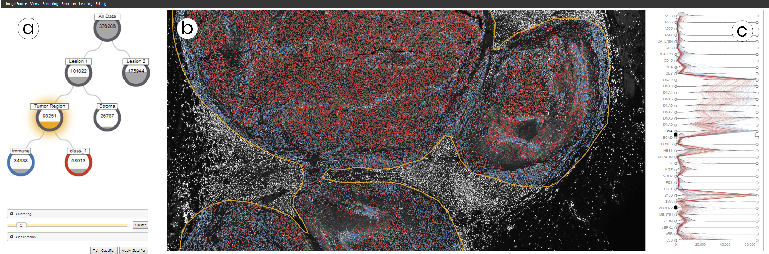
\includegraphics[width=\textwidth]{figures/system-examples/facetto_fig1_abc.pdf}
  \caption{Facetto links tissue inspection to expert-guided phenotype analysis. The phenotype tree (a) records analytical subsets, the tissue view (b) displays clustering and classification results in their spatial context, and the ridgeplot (c) supports feature inspection and filtering. These coordinated views let scientists inspect computational groupings and choose the cells and features used in subsequent analysis. Selected panels from Krueger et al.~\cite{AnchorFacetto}, Fig.~1(a--c); cropped from the original.}
  \label{fig:facetto-interface}
\end{figure*}


Metis places feedback at another point in analysis. Medicinal chemists evaluate generated molecules and identify favorable or unfavorable substructures. ~\cite{AnchorMetis} The system can fit a reward model to overall preferences or construct a reward function from supported feedback for integration into a configured REINVENT generation loop. The chemist supplies evaluations and initiates another run; some recorded feedback is not incorporated into generation. Compared with Facetto’s phenotype assignments, the affected objects are generated molecular candidates. The scientist influences which possibilities are produced or favored, rather than only interpreting an existing result.

% Requires graphicx. Permission status: unconfirmed; see README.
\begin{figure}[t]
  \centering
  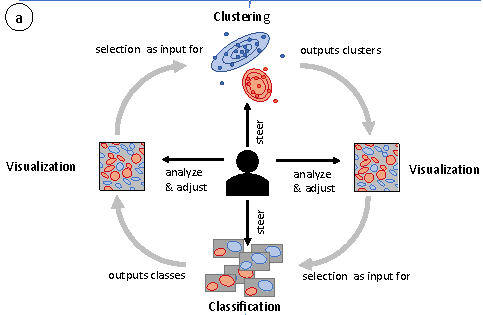
\includegraphics[width=\linewidth]{figures/system-examples/facetto_fig8a_loop.pdf}
  \caption{Facetto couples clustering and classification through an expert-guided analysis loop. Scientists inspect and adjust the visualized results, then select subsets that become inputs to the next computational step. The paper describes using labeled cells to train a classifier and clustering classification results to investigate further subgroups, connecting Algorithmic organization with Adaptive learning from expert input. Source: Krueger et al.~\cite{AnchorFacetto}, Fig.~8(a); cropped from the original.}
  \label{fig:facetto-learning-loop}
\end{figure}


Context-conditioned assistance does not need to learn a persistent user model. ExaViz computes viewpoints and paths from molecular geometry and a selected target, illustrating system-selected guidance rather than merely applying an entered camera position.~\cite{MapExaViz} SAMIRA conditions retrieved references and guidance on the current patient slice and spoken request; point-prompt segmentation corrections alone are not the basis for its Adaptive placement.~\cite{MapSAMIRA} The patient-health dashboard automatically selects visual modules from task and data characteristics, a narrower form of data-conditioned adaptive presentation rather than learned clinician personalization.~\cite{MapDashboard} These interpretations concern implemented selection of assistance; replay alone, fixed opacity weighting, and proposed future personalization do not establish the same contribution.

Facetto and Metis connect algorithmic processing with adaptation through analyst feedback. Facetto illustrates expert-directed analysis through guided cases, while Metis implements a feedback mechanism without reporting a participant outcome study. Their benefits therefore warrant evaluation at the task level: do revised outputs better serve the analyst’s goals, and can the analyst correct an inappropriate adjustment? Such evaluation should distinguish temporary concerns from lasting preferences and examine whether repeated prioritization limits exploration.

The feedback loop also changes the meaning of later signals. A recommendation can influence the next selection, which may then be treated as evidence of an enduring preference. Evaluating the inferred state independently of that influence is therefore important. The task determines what is at stake: a suggested region affects navigation, a propagated label changes a selection, and prioritized comparisons influence which explanations receive attention. Errors cannot be ranked by task name alone; a seemingly local selection error can propagate into subsequent comparisons and conclusions. Section~\ref{sec:evaluation} examines these consequences through intent accuracy, exploration breadth, appropriate reliance, and recovery rather than treating adaptation as a single performance score.

Further examples delimit responsive intervention. In interactive VR annotation, corrective positive and negative clicks trigger revised whole-volume segmentation.~\cite{ExpandedE24} Liver MR navigation uses newly acquired surface evidence to correct deformation of the preoperative model.~\cite{ExpandedE15} ASCRIBE-XR resolves underspecified segmentation, resolution, and meshing choices within a language-driven workflow; its Adaptive interpretation is limited to this context-conditioned selection, not learned personalization.~\cite{ExpandedE28} Fixed-threshold QC alerts and explicitly weighted aneurysm retrieval remain Algorithmic here.~\cite{ExpandedE48,ExpandedE46}

\subsection{Conversational Assistance and Agentic Orchestration}
\label{sec:assistance-conversational}

Conversational assistance changes the way analytic intent enters a computational workflow. A literal spoken command may duplicate a button, whereas a request to compare observations can require resolving entities, selecting data, constructing operations, and choosing a representation. The latter transfers some operational decisions to the system. Its scope depends on the implemented workflow: language input does not by itself establish autonomous planning, and a fluent explanation does not demonstrate correct execution.

FathomGPT connects natural-language questions about ocean data to scientific-name resolution, SQL generation and execution, and visual or image results. Conversation history supports refinement, while inspectable SQL exposes an intermediate representation of the requested operation.~\cite{AnchorFathomGPT} The scientist specifies a question and assesses the response; computation supplies steps that would otherwise require explicit query construction. This combines Conversational assistance with Algorithmic operations. It also illustrates bounded orchestration: the consequential delegation lies in translating a request into an executable sequence, without implying unrestricted system authority over scientific interpretation.

% Requires graphicx; uses the existing AnchorFathomGPT bibliography entry.
% Place fathomgpt_observer_map.png in figures/.
% Publication reuse permission remains unconfirmed; see README.md.
\begin{figure}[t]
  \centering
  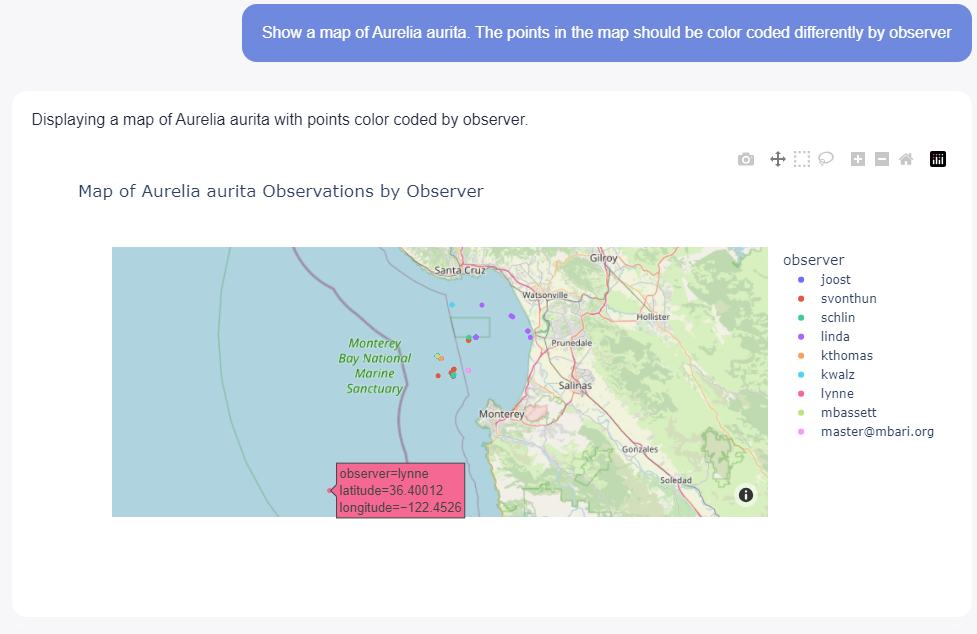
\includegraphics[width=\linewidth]{figures/system-examples/fathomgpt_observer_map.png}
  \caption{FathomGPT translates a natural-language request into an interactive map of \textit{Aurelia aurita} observations, with points colored by observer. The scientist specifies the species and grouping, while the system constructs the visualization; hovering reveals the observer and coordinates of an individual record. This connects Conversational assistance to spatial comparison and inspection of observation metadata on a Desktop/Planar display. Source: Khanal et al.~\cite{AnchorFathomGPT}, Fig.~12. Copyright 2024 held by the owner/author(s).}
  \label{fig:fathomgpt-observer-map}
\end{figure}


PhenoFlow provides a clinical counterpart: natural-language cohort requests are translated into data-wrangling code, accompanied by explanations and field-level views that neurologists can inspect.~\cite{EvalKim2025} Its model receives dataset metadata, including field names and coding information, rather than raw patient records. This bounds the translation mechanism; it does not remove the need to check whether the available fields support the intended cohort. FathomGPT and PhenoFlow thus make intermediate operations available for inspection while leaving scientific interpretation to the analyst.

General visual analytics examples expose further distinctions. LightVA separates planning, execution, and coordination, with on-demand task decomposition and opportunities to modify task flow.~\cite{LightVA} CausalChat represents proposed causal relationships and distinguishes LLM-suggested links that are not confirmed by data.~\cite{CausalChat} ProactiveVA instead uses interaction history and notes to infer possible needs and offer assistance.~\cite{EvalZhao2025} These illustrate workflow planning, hypothesis proposal, and context-dependent initiative, respectively; they are not interchangeable evidence of autonomous scientific reasoning. Their role here is contextual comparison, not automatic inclusion in the life-science corpus. A proposed causal link remains a hypothesis, and a plausible plan still requires examination of its operations and evidence.

Robin supports language-mediated comparison of genomic loop-caller outputs.~\cite{ExpansionX018} Users upload results generated by external loop-calling tools and inspect them through HiGlass, an integrated viewer for genomic contact maps. This separation makes the provenance boundary consequential: an explanation of uploaded results should remain distinguishable from execution of the analysis that produced them. A conversational interface does not erase that division of responsibility or establish adaptive intervention.

The contrast with Metis clarifies what interaction changes. A FathomGPT follow-up can revise a query or presentation; Metis feedback can alter the scoring or learning process that shapes later molecular candidates. Both accept high-level human guidance, but neither conversational continuity nor feedback collection alone establishes a persistent, accurate model of a scientist's goals. Inspection must address the relevant transformation: which data and operations a request selected, or how feedback affected subsequent outputs. Evaluation consequently needs to test whether a generated query represents the intended question and, for feedback-driven generation, whether candidate changes reflect the supplied feedback and remain open to correction.

FathomGPT's prompt-level evaluation supports successful interpretation and execution within its tested setting. Scientific conclusions drawn from a generated view additionally require examination of the data and assumptions behind the analysis. Analysts need to distinguish an account of an operation from its inputs, executed transformations, and results, using the provenance and control mechanisms discussed in Section~\ref{sec:evaluation}. The benefit of expressing intent in language must be considered alongside the work of verifying how that intent was operationalized.

\subsection{Immersive Assistance: Computational Use of Spatial Context}
\label{sec:assistance-immersive}

Immersive assistance uses spatial or embodied context, such as gaze, gesture, viewpoint, or body position, to guide computational support for an analytical task. The system interprets these signals to select, constrain, or adjust an operation: a spatial sketch, for example, can specify constraints that guide the generation of candidate molecular structures.

NUI-VR$^2$ couples VR gesture and voice interaction to segmentation and inspection of medical volumes. Seeds and parameters enter routines that compute probability maps and use feature selection; the resulting boundaries and volume views can then be examined.~\cite{AnchorNUIVR} The substantive assistance lies in the segmentation computation. Its spatial interface establishes VR use, but does not on its own demonstrate context-sensitive guidance, preference learning, or a separate Immersive assistance mechanism. Reported segmentation comparisons assess output behavior rather than establishing a general advantage for embodied interaction.

ProteinSketch provides a more direct connection between spatial expression and computational assistance. Users sketch secondary structures and volumes, providing spatial constraints for structure generation, sequence design, prediction, and filtering. ~\cite{AnchorProteinSketch} Spatial specification helps define a design space within which algorithms generate candidates. This coupling supports an Immersive interpretation alongside Algorithmic assistance: spatial input contributes analytically through its translation into computational constraints. The scientist specifies and interprets structures, while the pipeline supplies candidates that meet its implemented objectives. The preprint's computational and laboratory results support design feasibility; they do not isolate improved designer performance attributable to VR. Section~\ref{sec:modality} considers these environmental conditions separately from the mechanisms they host.

% Requires graphicx. Keep these PNGs alongside the manuscript, or adjust paths.
% Existing bibliography key: AnchorProteinSketch.
% DRAFT: confirm crop/publication reuse permission before submission.
\begin{figure*}[t]
  \centering
  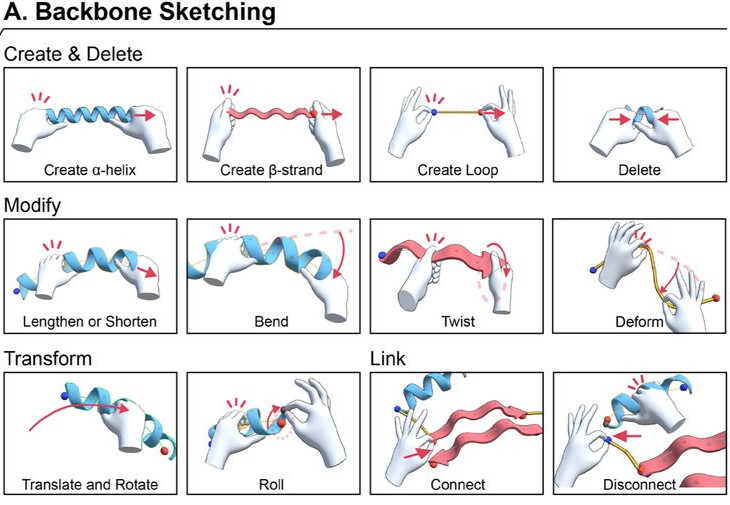
\includegraphics[width=0.64\textwidth]{figures/system-examples/proteinsketch_backbone_crop.png}\\[5pt]
  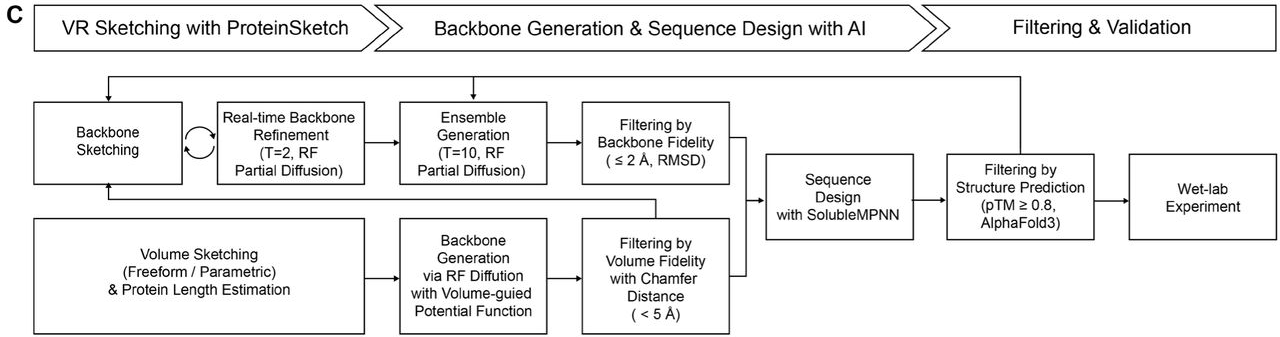
\includegraphics[width=\textwidth]{figures/system-examples/proteinsketch_workflow_crop.png}
  \caption{ProteinSketch connects spatial specification to generative protein design. (A) Two-handed gestures create, reshape, and connect secondary-structure elements in VR. (C) Backbone sketches and volumetric constraints feed computational refinement, generation, sequence design, and filtering. Scientists specify the desired geometry while computational models propose and evaluate candidate structures, linking Immersive and Algorithmic assistance within the design workflow. Selected panels cropped from Ma et al.~\cite{AnchorProteinSketch}, Fig.~1; original panel labels retained.}
  \label{fig:proteinsketch-workflow}
\end{figure*}


Spatial language creates a related requirement: a reference must resolve to identifiable data and an inspectable operation. Section~\ref{sec:modality-vr} contrasts elicited spatial-language requirements with implemented scene operations, keeping both distinct from demonstrated scientific reasoning.


The distinction also limits immersive-assistance claims. Vitessce Link synchronizes selection and other interaction state between mixed-reality and planar clients. Synchronization alone does not establish Immersive assistance, but its hand-controlled measurement tool provides a more specific mechanism: tracked finger positions define endpoints for measuring distances within a tissue map, with applications described for kidney and melanoma structures.~\cite{ExpansionX015} This supports Algorithmic assistance through geometric measurement and a narrowly scoped Immersive placement through embodied specification of that
computation; it does not establish Adaptive assistance or independently validated improvements in analytical performance. Similarly, moleculARweb's implemented SAXS-profile comparison, contact/linker analysis, and constrained molecular mechanics support narrowly scoped analytical functions. ~\cite{ExpansionX012,ExpansionX128}


\subsection{Overlapping Modes and Shifts in Analytic Agency}
\label{sec:assistance-overlap}

Assistance modes combine as analytical work moves between scientists and computational mechanisms. In Facetto, computational organization supports inspection, and expert-provided labels then guide classification. In FathomGPT, linguistic interpretation translates a request into operations whose visual results inform the analyst's next question. In ProteinSketch, scientists express spatial constraints that guide generative computation. Each transition connects a human judgment to a computational contribution and creates an opportunity to inspect the resulting evidence.

Agentic orchestration can plan and coordinate such operations, determining their sequence and how results pass between them. A workflow might combine conversational specification, algorithmic execution, and adaptive suggestions, with distinct opportunities for intervention at each stage. Scientists may revise the initial request, inspect an intermediate result, or redirect a proposed next step. These shifts concern the operational questions in Section~\ref{subsection:locusofagency}: proposal, scope, execution, assessment, and opportunities for inspection and revision. Different participants or computational components can take responsibility for these actions at different points in the workflow.

Clinical registry tools illustrate another division of work. StoryboardR organizes recorded events for visual interpretation, whereas REDCap's generative features can produce a textual summary of report data.~\cite{MillerShalhout2023StoryboardR,Shyr2026REDCapAI} The former delegates presentation; the latter also delegates an interpretive account that the researcher must check. Sections~\ref{sec:modality-desktop} and~\ref{sec:evaluation-effectiveness} examine the interface and evaluation consequences.

These shifts provide a basis for comparing combined assistance: which decisions scientists make directly, which they express through constraints or feedback, and which they delegate to computation. Effective support depends on matching those arrangements to the task and providing ways to inspect and revise consequential outputs. The next section examines how visualization modalities shape these opportunities; Section~\ref{sec:evaluation} considers the evidence needed to establish their analytical benefits.
